\documentclass[12pt]{book}
%Use apacite package for apa7 compatible reference style
\usepackage[natbibapa]{apacite}

\usepackage{colortbl}
\setlength{\parindent}{0pt}

\usepackage[a4paper,left=3cm,right=2.5cm,top=3cm,bottom=3cm, twoside]{geometry}
\usepackage[dvipsnames]{xcolor}
\usepackage{stmaryrd}
%%\usepackage{amssymb}
%%\usepackage{amsmath}
\usepackage{libertine}
\usepackage{caption}
\usepackage{subcaption}
\usepackage{float}
\usepackage{multirow}
\usepackage{tikz}
\usepackage{enumitem}
\usepackage{epigraph}

\usepackage{lscape}
\usepackage{titletoc}

\usepackage{booktabs}
\usepackage{arydshln}
\usepackage[nonumberlist]{glossaries}
\usepackage{calc}
\usepackage[]{titlesec} 
\definecolor{linkColor}{HTML}{32a852}
\usepackage[colorlinks=true,citecolor=linkColor,linkcolor=black]{hyperref}
\usepackage{fancyhdr}
\usepackage{lipsum}
\usepackage[en-US]{datetime2}
\usepackage{hyperref}

%%\usepackage{url}
\makeatletter
\newcommand\footnoteref[1]{\protected@xdef\@thefnmark{\ref{#1}}\@footnotemark}
\makeatother
\usepackage{footmisc}
\usepackage{doi}
\renewcommand{\doitext}{}%removes double doi!!

%\usepackage{zref-xr,zref-user}
\usepackage{nameref}
\usepackage{zref-xr}

%% \usepackage{float} % this was already imported!
\usepackage{longtable}
\usepackage{tabularray} %MB: better package for tables <3

% no hyphenation!!!
\tolerance=1
\emergencystretch=\maxdimen
\hyphenpenalty=100000
\hbadness=100000
\usepackage{nicematrix}
\usepackage{setspace}
\usepackage{lipsum}
\usepackage{gb4e} % for examples and glosses
\noautomath % needed for gb4e to work with bibtex

%%%%%%%%%%%%%%%%%%%%%%%%%%%%%%%%%%%%%%%%%%%%%%%%%%%%%%%%%%%%%%%%%%%%%%%%%%%%%%%%%%%%%%%%%%%%%%%%%%%%%%%%%%%%%%%%%%%%%%%%%%%%%%%%%%%%%%%%%%%%%%%%%%%%

\definecolor{yourcolor}{HTML}{8a0e19}%{008bb2}

\titleformat{\chapter}[display]
{\normalfont\color{yourcolor}}
{\filcenter\huge\color{black}\textsc\chaptertitlename\hspace*{2mm}%
	\begin{tikzpicture}[baseline={([yshift=-.6ex]current bounding box.center)}]
		\node[text=black] {\thechapter};
	\end{tikzpicture}
}
{1ex}
{\titlerule[1.5pt]\vspace*{1.5ex}\Huge\color{black}\textsc}
[]

\titleformat{name=\chapter,numberless}[display]
{\normalfont\color{black}}
{}
{1ex}
{\vspace*{-5cm}\Huge\textsc}
[]

\fancyhead{} % clear the headers
\fancyhead[L]{\nouppercase{\leftmark}}
\renewcommand{\chaptermark}[1]{\markboth{\chaptername\ \thechapter\ -- #1}{}}

\newcommand{\HRule}{\rule{\linewidth}{0.7mm}}
\newcommand{\Hrule}{\rule{\linewidth}{0.3mm}}

%%%%%%%%%% Fonts!!

\usepackage{fontspec}
\defaultfontfeatures{Mapping=tex-text} % to support TeX conventions like ``---''
\usepackage{xunicode} % Unicode support for LaTeX character names (accents, European chars, etc)
\usepackage{graphicx}
\usepackage{xltxtra} % Extra customizations for XeLaTeX

%\setmainfont{professionalfonts}
%\setmainfont{Charis SIL} 

%\usepackage{libertinus}
%\usepackage{ebgaramond}
%\setmainfont{Garamond}

\setmainfont{Libertinus Serif}
\newfontfamily\IPA{Doulos SIL}

\newfontfamily\typewriting{CMU Typewriter Text Regular}

\makeatletter
\renewcommand\tableofcontents{%
	\@starttoc{toc}%
}
\makeatother
\let\cleardoublepage=\clearpage
%%%%%%%%%%%%%%%%%%%%%%%%%%%%%%%%%%%%%%%%%%%%%%%%%%%%%%%%%%%%%%%%%%%%%%%%%%%%%%%%%%%%%%%%%%%%%%%%%%%%%%%%%%%%%%%%%%%%%%%%%%%%%%%%%%%%%%%%%%%%%%%%%%%%%%%

%%%%%%%%%%%%%%%%%%%%%%%%%%%%%%%%%%%%%%%%%%%%%%%%%%%%%%%%%%%%%%%%%%%%%%%%%%%%%%%%%%%%%%%%%%%%%%%%%%%%%%%%%%%%%%%%%%%%%%%%%%%%%%%%%%%%%%%%%%%%%%%%%%%%%%%

\setcounter{secnumdepth}{3}
\setcounter{tocdepth}{3}

\begin{document}	
	%% \begin{titlepage}
	%% 	\begin{center}
	%% 	
\includegraphics[height=2.2cm, width = 5cm]{images/PGSL.png}
        %%         
\includegraphics[height=1.7cm, width = 5cm]{images/SHS.jpg} 
        %%         \hspace*{5pt}
        %%         %\includegraphics[height=1.7cm, width = 5cm]{images/HTL.png}
        %%         
\includegraphics[height=1.7cm, width = 5cm]{images/LLF.jpg}
	%% 	\end{center}
		
	%% 	\vspace*{10pt}
		
	%% 	\begin{center}
	%% 		%this page reamins in French! Simply add the name of your discipline and strand.
	%% 		% e.g., Sciences du langage, Parcours Linguistique Théorique et Expérimentale
	%% 	{\LARGE \textbf{AVERTISSEMENT}}
	%% 	\end{center}
		
		
	%% 	{\Large 
	%% 	Ce mémoire est le fruit d’un travail approuvé par le jury de soutenance et réalisé dans le but d’obtenir le diplôme de Master\textbf{ [Mention et Parcours à renseigner]}. Ce document est mis à disposition de l’ensemble de la communauté universitaire élargie.
	%% 	Il est soumis à la propriété intellectuelle de l’auteur. Ceci implique une obligation de citation et de référencement lors de l’utilisation de ce document.
	%% 	D’autre part, toute contrefaçon, plagiat, reproduction illicite encourt toute poursuite pénale.}

        %%         \vspace*{300pt}
		
	%% 	Code de la Propriété Intellectuelle. Articles L 122.4\\		
	%% 	Code de la Propriété Intellectuelle. Articles L 335.2 - L 335.10
	%% \end{titlepage}		


	%% \begin{titlepage}
	%% 	\begin{center}
	%% 	
\includegraphics[height=2.2cm, width = 5cm]{images/PGSL.png}
        %%         
\includegraphics[height=1.7cm, width = 5cm]{images/SHS.jpg} 
        %%         \hspace*{5pt}
        %%         %\includegraphics[height=1.7cm, width = 5cm]{images/HTL.png}
        %%         
\includegraphics[height=1.7cm, width = 5cm]{images/LLF.jpg}
	%% 	\end{center}
			
	%% 	\vspace*{10pt}
                
	%% 	\begin{center}
	%% 		{\Large \textbf{UNIVERSITÉ PARIS CITÉ}}\\
	%% 					\vspace*{10pt}
	%% 		{\large Faculté Sociétés et Humanités}\\
	%% 					\vspace*{10pt}
	%% 		{\large \textbf{UFR LINGUISTIQUE}}\\
	%% 					\vspace*{10pt}
	%% 					%replace by the name of the laboratory where you have done your research internship
	%% 	\textbf{	{\large Laboratoire de linguistique formelle (LLF)}}
	%% 	\end{center}
		
	%% 	\vfill
		
	%% 	\begin{center}
	%% 		\begin{tabular}{lr}
	%% 			Year [To add in YYYY format] &  N° [To add or not according to usage]\\
	%% 		\end{tabular}
			
	%% 		Thesis for the diploma \textbf{[Add the title of the diploma [master 2 – mention + strand]]}
			
	%% 		Presented and defended publicly on: \textbf{[Add the date in the format DD Month YYYY]}
			
	%% 		\vspace*{20pt}
	%% 		By\\
	%% 		\vspace*{10pt}
	%% 		\textbf{		First name SURNAME}
			
	%% 		\vfill
			
	%% 		{ \Large \bfseries [Dissertation title: subtitle]}
	%% 		\vspace*{20pt}
            
	%% 		{ \large Under the supervision of Mr. [or Mrs] the Professor [or Doctor] [First-name Surname]}
			
	%% 		\vspace{1cm}
	%% 	\end{center}
		
	%% 	\vspace{1cm}
	%% 	\begin{center}
	%% 		JURY
	%% 	\end{center}
					
	%% 	\begin{center}
	%% 		\begin{tabular}{lll}
	%% 			Mr [or Mrs] the Professor [or Doctor] [First-name Surname] & \hspace*{40pt} & President  \\				
	%% 			Mr [or Mrs] the Professor [or Doctor] [First-name Surname] & \hspace*{40pt} & [quality]  \\				
	%% 			Mr [or Mrs] the Professor [or Doctor] [First-name Surname] & \hspace*{40pt} & [quality]  \\				
	%% 			Mr [or Mrs] the Professor [or Doctor] [First-name Surname] & \hspace*{40pt} & [quality]  \\				
	%% 			Mr [or Mrs] the Professor [or Doctor] [First-name Surname] & \hspace*{40pt} & [quality]  \\				
	%% 		\end{tabular}\\[1cm]
	%% 	\end{center}
		
	%% 	\newpage
	%% \end{titlepage}
	
	\pagestyle{fancy}
	\fancyhead{}
	\renewcommand{\chaptermark}[1]{\markboth{\textsc{#1}}{}}
        \frontmatter
        
	%% \phantomsection
\chapter*{Acknowledgments}\label{chap:Acknowledgments}
\addcontentsline{toc}{chapter}{Acknowledgments}


\textit{\textbf{To Mr [or Mrs] the Professor [or Doctor] [First-name Surname]}, Title Discipline, Title Discipline, Title Discipline, Title Discipline, Title Discipline, Title Discipline…}\\

 \setlength{\parindent}{1cm}
Lorem ipsum dolor sit amet, consetetur sadipscing elitr, sed diam nonumy eirmod tempor invidunt ut labore et dolore magna aliquyam erat, sed diam voluptua. No sea sanctus est.\\
 \setlength{\parindent}{0cm}


\textit{\textbf{To Mr [or Mrs] the Professor [or Doctor] [First-name Surname]}, Title Discipline, Title Discipline, Title Discipline, Title Discipline, Title Discipline, Title Discipline…}\\

 \setlength{\parindent}{1cm}
Lorem ipsum dolor sit amet, consetetur sadipscing elitr, sed diam nonumy eirmod tempor invidunt ut labore et dolore magna aliquyam erat, sed diam voluptua. No sea sanctus est.\\
 \setlength{\parindent}{0cm}


\textit{\textbf{To Mr [or Mrs] the Professor [or Doctor] [First-name Surname]}, Title Discipline, Title Discipline, Title Discipline, Title Discipline, Title Discipline, Title Discipline…}\\

 \setlength{\parindent}{1cm}

Lorem ipsum dolor sit amet, consetetur sadipscing elitr, sed diam nonumy eirmod tempor invidunt ut labore et dolore magna aliquyam erat, sed diam voluptua. No sea sanctus est.\\
 \setlength{\parindent}{0cm}


\textit{\textbf{To Mr [or Mrs] the Professor [or Doctor] [First-name Surname]}, Title Discipline, Title Discipline, Title Discipline, Title Discipline, Title Discipline, Title Discipline…}\\

 \setlength{\parindent}{1cm}
Lorem ipsum dolor sit amet, consetetur sadipscing elitr, sed diam nonumy eirmod tempor invidunt ut labore et dolore magna aliquyam erat, sed diam voluptua. No sea sanctus est.\\
 \setlength{\parindent}{0cm}


\textit{\textbf{To Mr [or Mrs] the Professor [or Doctor] [First-name Surname]}, Title Discipline, Title Discipline, Title Discipline, Title Discipline, Title Discipline, Title Discipline…}\\

 \setlength{\parindent}{1cm}

Lorem ipsum dolor sit amet, consetetur sadipscing elitr, sed diam nonumy eirmod tempor invidunt ut labore et dolore magna aliquyam erat, sed diam voluptua. No sea sanctus est.\\
 \setlength{\parindent}{0cm}


        %% \phantomsection
\chapter*{Résumé et indexation en français}\label{chap:Résumé}
\addcontentsline{toc}{chapter}{Résumé et indexation en français}

Titre : sous-titre

Résumé : [=> se référer aux préconisations de l’équipe pédagogique : entre 1 700 signes et 4 000 signes]

Lorem ipsum dolor sit amet, consetetur sadipscing elitr, sed diam nonumy eirmod tempor invidunt ut labore et dolore magna aliquyam erat, sed diam voluptua. At vero eos et accusam et justo duo dolores et ea rebum. Stet clitaLorem ipsum dolor sit amet, consetetur sadipscing elitr, sed diam nonumy eirmod tempor invidunt ut labore et dolore magna aliquyam erat, sed diam voluptua. At vero eos et accusam et justo duo dolores et ea rebum. Stet clita kasd gubergren, no sea takimata sanctus est Lorem ipsum dolor sit amet. Lorem ipsum dolor sit ametLorem ipsum dolor sit amet, consetetur sadipscing elitr, sed diam nonumy eirmod tempor invidunt ut labore et dolore magna aliquyam erat, sed diam voluptua. At vero eos et accusam et justo duo dolores et ea rebum. Stet clita kasd gubergren, no sea takimata sanctus est Lorem ipsum dolor sit amet. Lorem ipsum dolor sit ametLorem ipsum dolor sit amet, consetetur sadipscing elitr, sed diam nonumy eirmod tempor invidunt ut labore et dolore magna aliquyam erat, sed diam voluptua. At vero eos et accusam et justo duo dolores et ea rebum. Stet clita kasd gubergren, no sea takimata sanctus est Lorem ipsum dolor sit amet. Lorem ipsum dolor sit amet kasd gubergren, no sea takimata sanctus est Lorem ipsum dolor sit amet. Lorem ipsum dolor sit amet. Lorem ipsum dolor sit amet.
\\

Mots clés français : 
\\

Forme ou Genre : 
\\

fMeSH\footnote{Répertoire structuré de mots-clés pour l'analyse de contenu et le classement de documents dans le domaine biomédical (français/anglais)} : Dissertation universitaire
\\

Rameau\footnote{Répertoire d'autorité-matière encyclopédique et alphabétique unifié (français)} :  Thèses et écrits académiques 	











	%% \phantomsection
\chapter*{Abstract and indexation in English}\label{chap:abstract}
\addcontentsline{toc}{chapter}{Abstract and indexation in English}

Title: subtitle

Abstract: [=> verify with the pedagogical team: between 1 700 words and 4 000 characters]

Even though using "lorem ipsum" often arouses curiosity due to its resemblance to classical Latin, it is not intended to have meaning. Where text is visible in a document, people tend to focus on the textual content rather than upon overall presentation, so publishers use lorem ipsum when displaying a typeface or design in order to direct the focus to presentation. "Lorem ipsum" also approximates a typical distribution of spaces in English. Even though using "lorem ipsum" often arouses curiosity due to its resemblance to classical Latin, it is not intended to have meaning. Where text is visible in a document, people tend to focus on the textual content rather than upon overall presentation, so publishers use lorem ipsum when displaying a typeface or design in order to direct the focus to presentation. "Lorem ipsum" also approximates a typical distribution of spaces in English. Even though using "lorem ipsum" often arouses curiosity due to its resemblance to classical Latin, it is not intended to have meaning. Where text is visible in a document, people tend to focus on the textual content rather than upon overall presentation, so publishers use lorem ipsum when displaying a typeface or design in order to direct the focus to presentation. "Lorem ipsum" also approximates a typical distribution of spaces in English. 
\\


English keywords:	
\\


Publication type:
\\

MeSH : Academic Dissertation 





	%% \phantomsection
\chapter*{List of abbreviations}\label{chap:abbréviations}
\addcontentsline{toc}{chapter}{List of abbreviations}


\begin{itemize}
    \item LIDSA : Lorem Ipsum Dolor Sit Amet
    \item LIDSA : Lorem Ipsum Dolor Sit Amet
    \item LIDSA : Lorem Ipsum Dolor Sit Amet
    \item LIDSA : Lorem Ipsum Dolor Sit Amet
    \item LIDSA : Lorem Ipsum Dolor Sit Amet
    \item LIDSA : Lorem Ipsum Dolor Sit Amet
    \item LIDSA : Lorem Ipsum Dolor Sit Amet
    \item LIDSA : Lorem Ipsum Dolor Sit Amet
    \item LIDSA : Lorem Ipsum Dolor Sit Amet
    \item LIDSA : Lorem Ipsum Dolor Sit Amet
    \item LIDSA : Lorem Ipsum Dolor Sit Amet
    \item LIDSA : Lorem Ipsum Dolor Sit Amet
    \item LIDSA : Lorem Ipsum Dolor Sit Amet
    \item LIDSA : Lorem Ipsum Dolor Sit Amet
    \item LIDSA : Lorem Ipsum Dolor Sit Amet
    \item LIDSA : Lorem Ipsum Dolor Sit Amet
    \item LIDSA : Lorem Ipsum Dolor Sit Amet
    \item LIDSA : Lorem Ipsum Dolor Sit Amet
    \item LIDSA : Lorem Ipsum Dolor Sit Amet
\end{itemize}

	\pagebreak

	\tableofcontents{}
	\addcontentsline{toc}{chapter}{Table of content}
	
	\mainmatter
	
	\setlength{\parskip}{.7em}
	\titlespacing*{\section}{0pt}{.9em}{.8em}
	\renewcommand{\baselinestretch}{1.1}
	
	\fancyhead[RO]{\leftmark}
	\fancyhead[LE]{\textsc{\chaptername~\thechapter}}
	
	%% \phantomsection
\chapter*{Introduction}\label{chap:Introduction}
\addcontentsline{toc}{chapter}{Introduction}
\startcontents[chapters]

Language can be a surprisingly complex system, especially for something used by people every day with such ease. We generate complex structures with words linked to each other in intricate ways all the time and somehow other people manage to understand the meaning we try to convey through this whole system of communication.

Polish is an example of a language with a relatively free word order, therefore often the links between words are marked morphologically. Agreement between words is one of the ways to figure out if certain words are connected, which means the two words share a value of a certain feature they both have. Though it usually is very simple, sometimes agreement can be extremely convoluted. This study aims to investigate at least some of this complexity to help find ways to describe the agreement patterns and universalities between languages.

	
	\chapter{Theoretical background}
\startcontents[chapters]

\section{Grammatical gender in Polish}
There are multiple options of defining grammatical genders in Polish. The one chosen for this study was proposed by Mańczak (1956), where he differentiates between 5 genders:
\begin{itemize}
\item masculine personal
\item masculine animate
\item masculine inanimate
\item feminine
\item neuter
\end{itemize}
Saloni (1976) proposed an even more elaborate system, where he talked about 9 genders (instead of one neuter there were two and additionally there were three genders for plurale tantum nouns). Such a system is, however, not necessary for the current analysis, therefore we will adopt the 5 genders proposed by Mańczak. For ease of reference we will use for them the names that Saloni used, which are: M1 (masculine personal), M2 (masculine animate), M3 (masculine inanimate), F (feminine) and N (neuter).

The difference between the genders can be observed when looking at appropriate forms of adjectives in the accusative case. Adjectives agree their genders with nouns and the accusative case provides the most diversity in terms of gender forms.

The example presented here comes from Mańczak (1956). There will be 5 nouns and one adjective for all of them used as an example: \textsl{mężczyzna} (meaning 'man'), \textsl{pies} (meaning 'dog'), \textsl{stół} (meaning 'table'), \textsl{kobieta} (meaning 'woman'), \textsl{dziecko} (meaning 'child') and \textsl{dobry} (meaning 'good').

\begin{tblr}
  {
    hlines, vlines,
    cell{1}{1} = {r=2}{l},
    cell{2}{3} = {r=4}{l},
  }
  dobrego & mężczyznę & dobrych & mężczyzn & masculine personal \\
  dobrego & psa & dobre & psy & masculine animate \\
  dobry & stół & dobre & stoły & masculine inanimate \\
  dobrą & kobietę & dobre & kobiety & feminine \\
  dobre & dziecko & dobre & dzieci & neuter \\
\end{tblr}

\section{Previous work on hybrid agreement}

\section{Polish nouns with hybrid gender}
\subsection{Socially gendered nouns}
\subsection{Profession nouns}
\subsection{Depreciative forms of M1 nouns}

\section{Hypothesis}

	
	
\chapter{Methodology}

\startcontents[chapters]

\section{Agreement sources}
The corpus used for this study was the 300M subcorpus of the National Corpus of Polish \citep{przepiorkowski_narodowy_2012}, which was parsed using Trankit \citep{trankit}. The dependency trees (conforming to the Universal Dependency standard, henceforth UD) obtained this way were searched for words, which could trigger hybrid agreement: profession nouns, socially gendered nouns and depreciative forms of M1 nouns. The subsections below describe how those nouns were chosen.

\subsection{Profession nouns}
Nouns in this category came from two studies about feminitives in Polish. The first was a survey reported by \cite{szpyra-kozlowska_premiera_2019}, where participants were asked to create feminitives from 50 masculine nouns, that in modern Polish do not have feminine counterparts at all or those counterparts are rarely used. For each noun participants had the option to give no answer. The second study was an experiment conducted by \cite{szpyra-kozlowska_czy_2022}, where they tested whether certain feminitives are less accessible by asking participants to try to pronounce them. They chose 20 feminitives, which are formed from masculine nouns that end in consonant clusters such as /kt/, /tr/ or /rg/. According to \cite{klemensiewicz_tytuly_1957} adding the -ka suffix, the function of which can be to create the feminitve, makes the word difficult to pronounce. Those two studies give a list of 60 nouns in total, for which it is said to be difficult to form feminine counterparts. It is therefore likely that, if there was a female referent of a noun from this list, the masculine noun would be used, leading to hybrid agreement. 

Both of the studies determine in some way which of the tested nouns have less available feminitives than others: in \cite{szpyra-kozlowska_czy_2022} those are the nouns for which there are the highest error rates in pronunciation, whereas in \cite{szpyra-kozlowska_premiera_2019} -- the nouns for which the most people refused to propose a feminitive. Taking this approach has, however, two downsides: first, it requires an arbitrary threshold that separates the nouns that have an easily formed feminitive from the nouns for which creating the feminine counterpart is more difficult. Second, this approach significantly limits the number of nouns for analysis. Considering this, the current study used all of the nouns from the two studies on Polish feminitves.

For ease of reference, all of those nouns are called \textsl{profession} nouns, despite not all of them actually referring to professions. Meanings of all nouns are presented in Table \ref{tab:noun-translations} in the Appendix.

\subsection{Socially gendered nouns}
The nouns for this category were found using the Polish Academy of Sciences Great Dictionary of Polish available online.\footnote{https://wsjp.pl/} The advanced search option allowed to search for nouns in the thematic category \textsc{human as a physical being: human physicality: sex}. This search yielded 586 results, which then had to be manually filtered to find the nouns that only refer to humans (and not, for example, abstract nouns or nouns referring to body parts) and that had incongruent grammatical and semantic gender. The 19 nouns selected this way can be found in Table \ref{tab:noun-translations} in the Appendix.

\subsection{Depreciative forms}
For this category no list of nouns was created, since the corpus was annotated and it was possible to look up the depreciative forms by checking the words' morphological description. It is possible to create depreciative forms of surnames, however these were excluded from the analysis, because there was no way of determining the referents and therefore no way of ensuring that there is hybrid agreement. Surname \textsl{Machała} found in the corpus can serve as an example: let us say that the \textsl{Machała} family bought a new car. Assuming the family consists of at least one man, the speaker can use both (\ref{ex:Machałowie}) and (\ref{ex:Machały}) to convey that information, depending on their attitude they have towards the situation: (\ref{ex:Machałowie}) if the speaker is neutral or positive and (\ref{ex:Machały}) if they are negative. However, if there are only women in the family, the speaker can only use (\ref{ex:Machały}). Without the context it is unclear whether \textsl{Machały} in (\ref{ex:Machały}) is used as a depreciative or simply to refer to women and therefore we cannot decide if this is an example of hybrid agreement.

\begin{exe}
  \ex
  \begin{xlist}
    \ex\label{ex:Machałowie}
    \gll Machał-owie kupi-li nowe auto.\\
    Machała-pl.nom.m1.ndepr buy-3pl.m1.past new car\\
    \ex\label{ex:Machały}
    \gll Machał-y kupi-ły nowe auto.\\
    Machała-pl.nom.m1.depr buy-3pl.f.past new car\\
    \trans ``Machałas bought a new car.''
  \end{xlist}
\end{exe}

Morphological analyzer Morfeusz \citep{kieras_morfeusz_2017} can mark forms as surnames which made it easy to exclude them from the analysis. 

\subsection{Finding agreement sources in the corpus}
The code used for extracting corpus data in this study can be found in a GitHub repository.\footnote{https://github.com/bmagdab/hybrid-agreement} The general idea of how the code works is presented in this chapter.

After choosing the nouns to be searched in the corpus, it was necessary to find all of their forms and the forms' morphological descriptions, which was done using the morphological analyzer Morfeusz. First the corpus was searched for occurrences of nouns, which could be sources of hybrid agreement. Those nouns were saved if they were in the list of gendered or profession noun forms or if they were marked as depreciative in their morphological description. To ensure that no homonyms were accidentaly saved for later analysis, the morphological description of a found word was compared with the one given by Morfeusz. This way, for example, the word \textsl{premiera} was excluded if it was an instance of the lexeme \textsl{premiera}, meaning \textsl{premiere} but not if it was an instance of the lexeme \textsl{premier}, meaning \textsl{prime minister}, in the singular accusative form.

Once it was sure that the right noun was found, the dependency tree was searched for words that can agree their gender with that of the noun. This was the head of the noun (which could be an example of predicative agreement), adjectives attached to the noun (which could be examples of attributive agreement), and relative pronouns referring to the noun. Based on the UD annotation guidelines, all dependents of the word were searched for a dependency label with a subtype \textsc{:relcl}, which in the UD annotation scheme mark the head of the relative clause. The relative pronoun was attached to the head of the relative clause and had a UD feature \textsc{PronType=Rel}.\footnote{https://universaldependencies.org/workgroups/newdoc/relative\_clauses.html} Once the possible agreement targets were found, the data could be used to look for occurrences of gender agreement.

\section{Listing agreement occurrences}
To analyse hybrid gender agreement in the found examples, it is necessary to mark the alternative to the grammatical gender of each agreement source. For all profession nouns that alternative gender was feminine, because the only chance of hybrid agreement for those noun is when the gender of the referent is feminine. For socially gendered nouns the alternative gender was assigned depending on the lexeme.

Once the alternative gender was determined, it was necessary to exclude plural nouns for which the gender discrepancy was between feminine and neuter. This is because for all types of agreement tested here, the plural feminine and plural neuter forms of targets of agreement are syncretic, therefore there is no hybrid agreement in those cases. This happens, for instance, in (\ref{ex:plural-feminine-neuter}), where in singular ((\ref{ex:sg.n}) and (\ref{ex:sg.f})) there is a difference between the feminine and neuter forms of the word \textsl{młoda}. In plural (\ref{ex:pl}), however, the form is the same for both neuter and feminine, so hybrid agreement cannot be observed. Examples like this were therefore excluded.

\begin{exe}
  \ex\label{ex:plural-feminine-neuter}
  \begin{xlist}
    \ex\label{ex:sg.n}
    \gll młod-e dziewczę\\
    young-sg.n.nom girl.sg.n.nom\\
    \ex\label{ex:sg.f}
    \gll młod-a dziewczę\\
    young-sg.f.nom girl.sg.n.nom\\
    \ex\label{ex:pl}
    \gll młod-e dziewczę-ta\\
    young-pl.nom girl-pl.n.nom\\
    \trans ``young girl''
  \end{xlist}
\end{exe}

The next step was to find occurrences of different types of agreement. The predicative agreement of a given noun was found in its head on three conditions: first, dependency label between the noun and the head had to be \textsc{nsubj}, which is the UD label for nominal subjects. Second, the head had to be a verb that inflects for gender, which is only true for verbs annotated as past participles,\footnote{The annotation scheme used for NKJP uses the past participle label not only for past participles, but also for parts of past tense and conditional mood forms \citep{przepiorkowski_narodowy_2012}.} active and passive participles. Third, the noun has to be in the nominative case. This condition helps filter out situations where a numeral phrase is in subject position, because then the verb does not agree with the subject -- it is in 3rd person, singular and neuter form, regardless of the noun. Therefore, predicative agreement cannot be observed in those situations at all and they should be excluded.

The search was simpler with attributive and relative pronoun agreement. The only requirement for attributive agreement was that the word is an adjective, which was verified by looking for the tag \textsc{adj} in the morphological description of the dependent. As for relative pronouns, all of the ones found earlier were included in the analysis, unless they did not inflect for gender (which was the case, for example, for the word \textsl{gdzie}, meaning \textsl{where}). 

The sentence in (\ref{ex:agreement-extraction}) serves as an example of the process of extracting agreement described in this chapter. The word, which could trigger hybrid agreement (but here does not, since the referent is male) is \textsl{premierem}. There are two words in the sentence that agree with this word in terms of gender: \textsl{jedynym} and \textsl{który}. All of the information saved for each instance of agreement is shown below. 

% NKJP_1M: 3571
\begin{exe}
  \ex\label{ex:agreement-extraction}
  \gll Nie jest prawd-ą, że premier Jerzy Buzek jest jedyn-y-m- premier-em, któr-y wystąpi-ł w Senac-ie.\\
  not be.3sg.pres truth.f.sg-inst that prime.minister.sg.m1.nom Jerzy Buzek be.3sg.pres only-m1-inst-sg prime.minister.m1-sg.inst which-sg.nom.m1 appear-3sg.m1.past in senate.m2-sg.loc \\
  \trans ``It's not true, that prime minister Jerzy Buzek is the only one that has appeared in the Senate.''
\end{exe}

\begin{tblr}{
    hlines, vlines,
    cell{2}{1} = {r=5,c=1}{c},
    cell{7}{1} = {r=3,c=1}{c},
    cell{1,10}{1} = {c=2}{l},
    cell{2-6}{3} = {c=2}{l},
  }
  & & Occurrence 1 & Occurrence 2 \\
  source of agreement & form & premierem & \\
  & lexeme & premier & \\
  & morphological description & subst:sg:inst:m1 & \\
  & grammatical gender & m1 & \\
  & other gender & f & \\
  agreement target & form & jedynym & który \\
  & morphological description & adj:sg:inst:m1:pos & adj:sg:nom:m1:pos \\
  & gender & m1 & m1 \\
  type of agreement & & attributive & relative pronoun\\
\end{tblr}


	%% \chapter{Results}
\startcontents[chapters]

\section{Descriptive statistics}
The first hypothesis this study aims to test is: there is a monotonous shift from one value of gender to another when going from attributive, through predicate to relative pronoun agreement. Additionally, the hypothesis proposed with the definition of generalized semantic agreement will be tested, which is that split hybrids (here the depreciative forms) are less likely to have generalized semantic agreement than lexical hybrids (here the socially gendered nouns and profession nouns). Before those hypotheses are addressed, let us look at the dataset extracted from the corpus. 

A total of 199 927 observations of agreement have been collected, although a vast majority of them was agreement with profession nouns, for which it was impossible to clearly determine whether it was hybrid agreement or not, as this would require manually finding the referent of the noun from the context. Because of that, only profession nouns with feminine agreement were used in the analysis. The summary of the types of agreements and controllers found in the dataset is in Tables \ref{tab:summary-agreements} and \ref{tab:summary-controllers} respectively. 

\begin{table}
  \centering
  \begin{tblr}
    {
      hlines,vlines,
      row{1} = {gray9},
    }
  Type of agreement & N & Percentage \\
  attributive & 1873 & 52.627\% \\
  predicative & 1478 & 41.529\% \\
  relative pronoun & 208 & 5.844\% \\
  \end{tblr}
  \caption{Numbers and percentages of different types of agreement in the dataset.}
  \label{tab:summary-agreements}
\end{table}

\begin{table}
  \centering
  \begin{tblr}
    {
      hlines,vlines,
      row{1} = {gray9},
    }
  Type of controller & N & Percentage \\
  depreciative & 1040 & 29.222\% \\
  gendered & 807 & 22.675\% \\
  profession & 1712 & 48.103\% \\
  \end{tblr}
  \caption{Numbers and percentages of different types of controllers in the dataset.}
  \label{tab:summary-controllers}
\end{table}

First, we will look at proportions of semantic agreement with attributive, predicate and relative pronoun targets, which are visualized by Figure \ref{fig:proportions}. Semantic agreement was favored in predicate agreement with both depreciatives and socially gendered nouns. This is contrary to the hypothesis about monotonous shift from one value to another along the agreement hierarchy, but this will be further addressed in the next section.

\begin{figure}
  \centering
  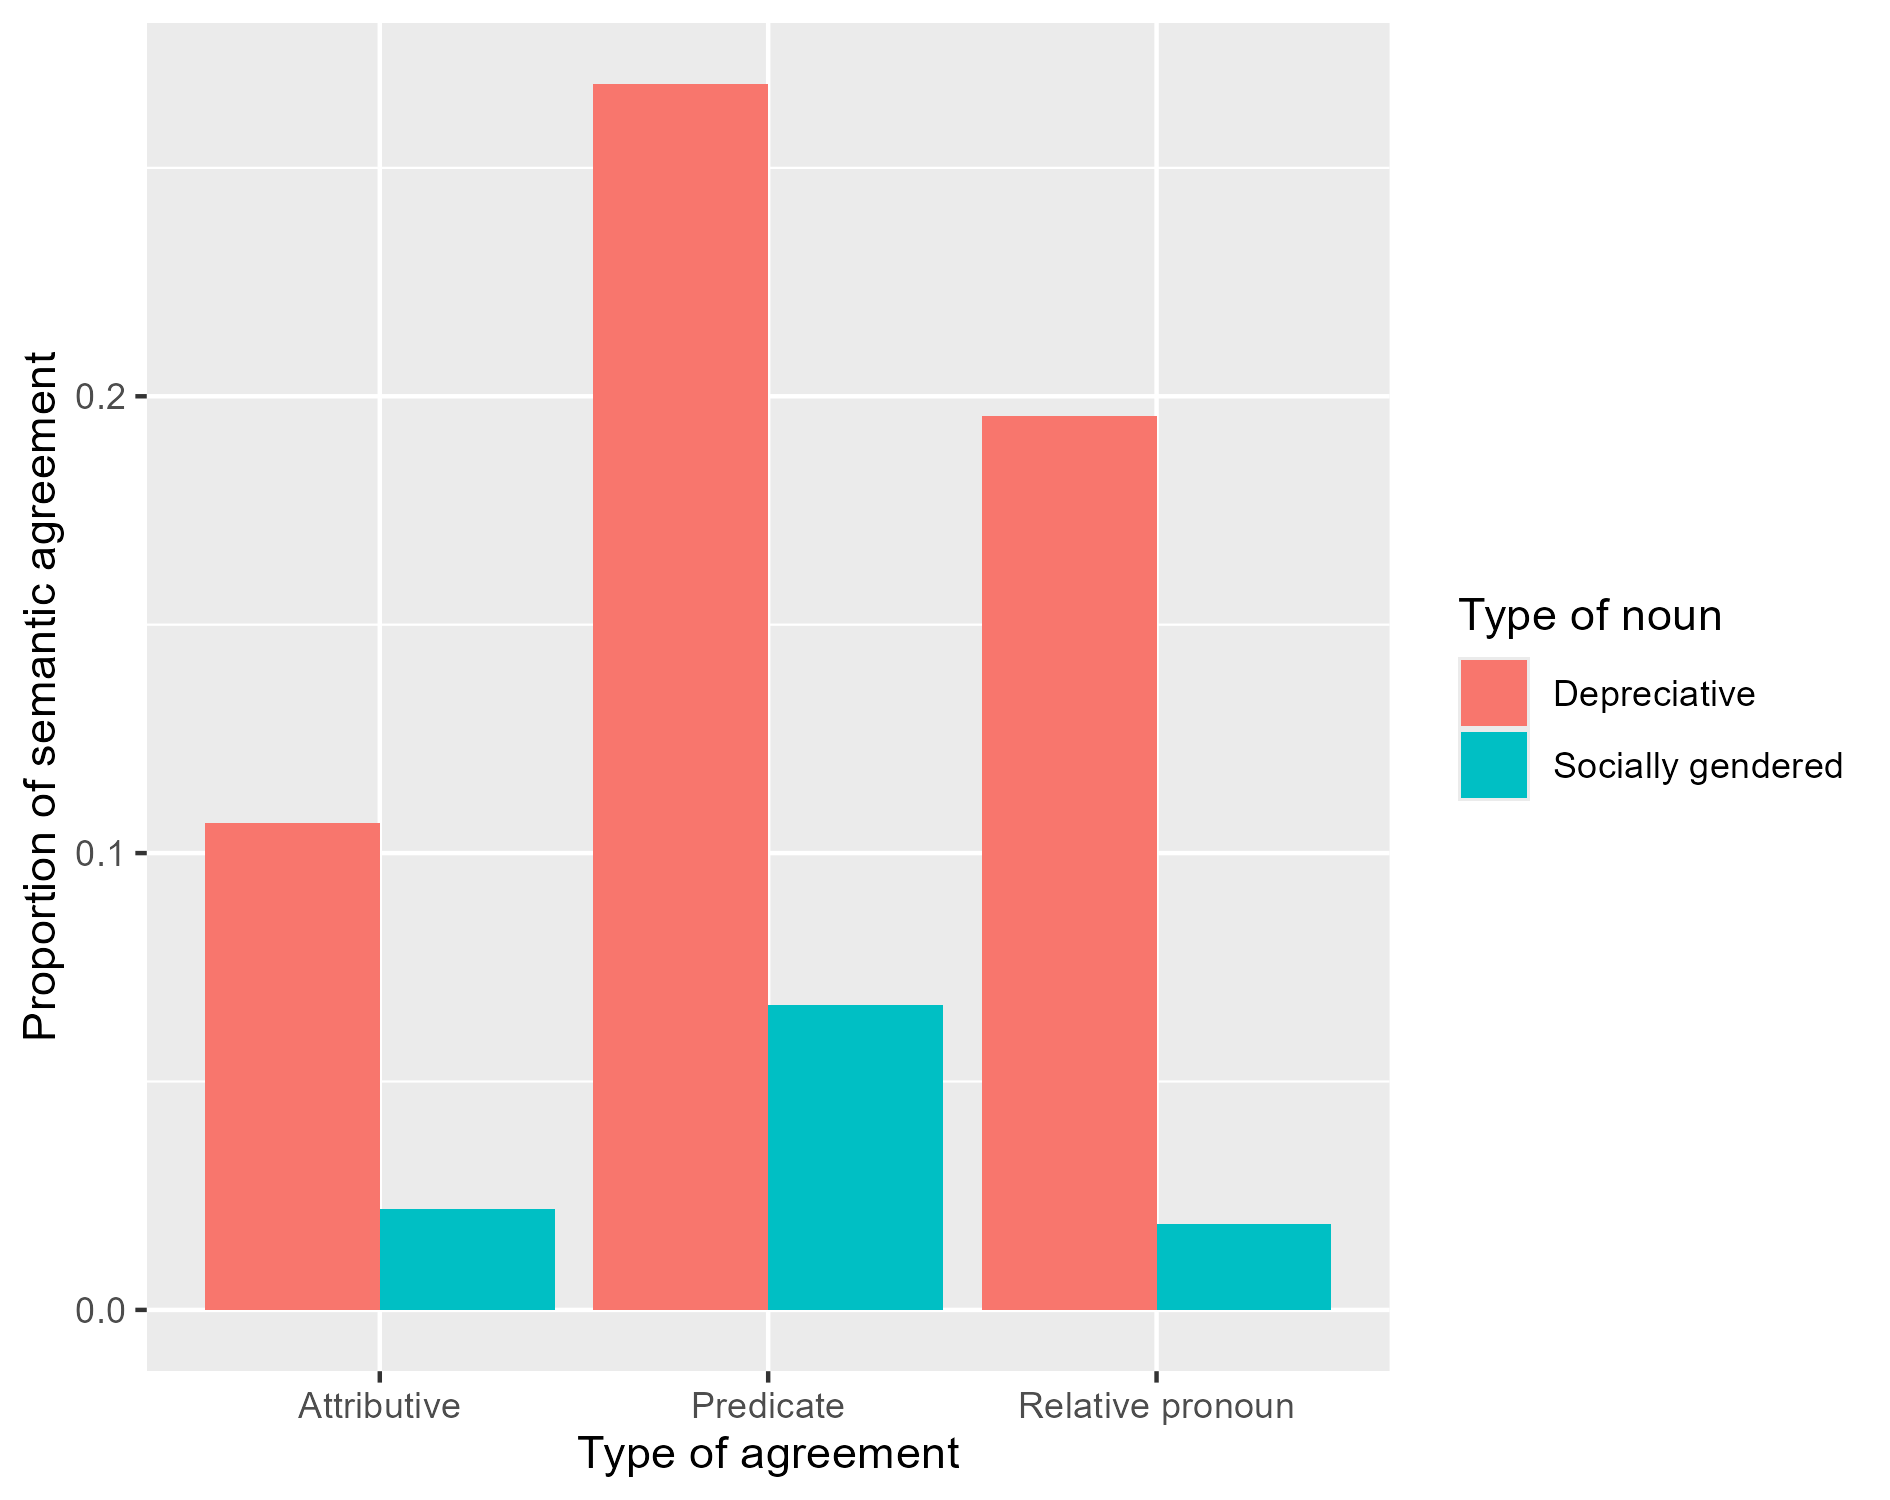
\includegraphics{images/props.png}
  \caption{Proportions of semantic agreement for each type of agreement for socially gendered and depreciative nouns.}
  \label{fig:proportions}
\end{figure}

For profession nouns only feminine agreement is considered, which means all of the examples have semantic agreement, so these occurrences cannot be reported in a similar figure. It can be reported, however, how many of the semantic agreement occurrences with profession nouns were attributive, predicate and relative pronoun agreement. This can be found in Table \ref{tab:prof-summary}. We can see a similar number of attributive and predicate, but very few relative pronoun agreements.

\begin{table}
  \centering
  \begin{tblr}
    {hlines, vlines,
    row{1} = {gray9}}
    Type of agreement & N & Percentage \\
    Attributive & 845 & 49.357\% \\
    Predicate & 758 & 44.276\% \\
    Relative pronoun & 109 & 6.367\% \\
  \end{tblr}
  \caption{Number of different types of agreement found with profession nouns along with their percentages among the semantic agreements with profession nouns}
  \label{tab:prof-summary}
\end{table}

Figure \ref{fig:distance} shows the average distance between the target and the controller of agreement measured as the number of intervening words. It was the largest in predicate agreement for both depreciatives and socially gendered nouns. The exact average distances can be found in Table \ref{tab:distance}. It was most common for attributive agreements to have the target before the controller (73.5\%), with predicate agreements it happened in 30.2\% of cases. There were 11 occurrences of target before controller in relative pronoun agreement, but those have been a result of parsing errors since it it not possible to put a relative pronoun before the noun to which it refers. 

\begin{figure}
  \centering
  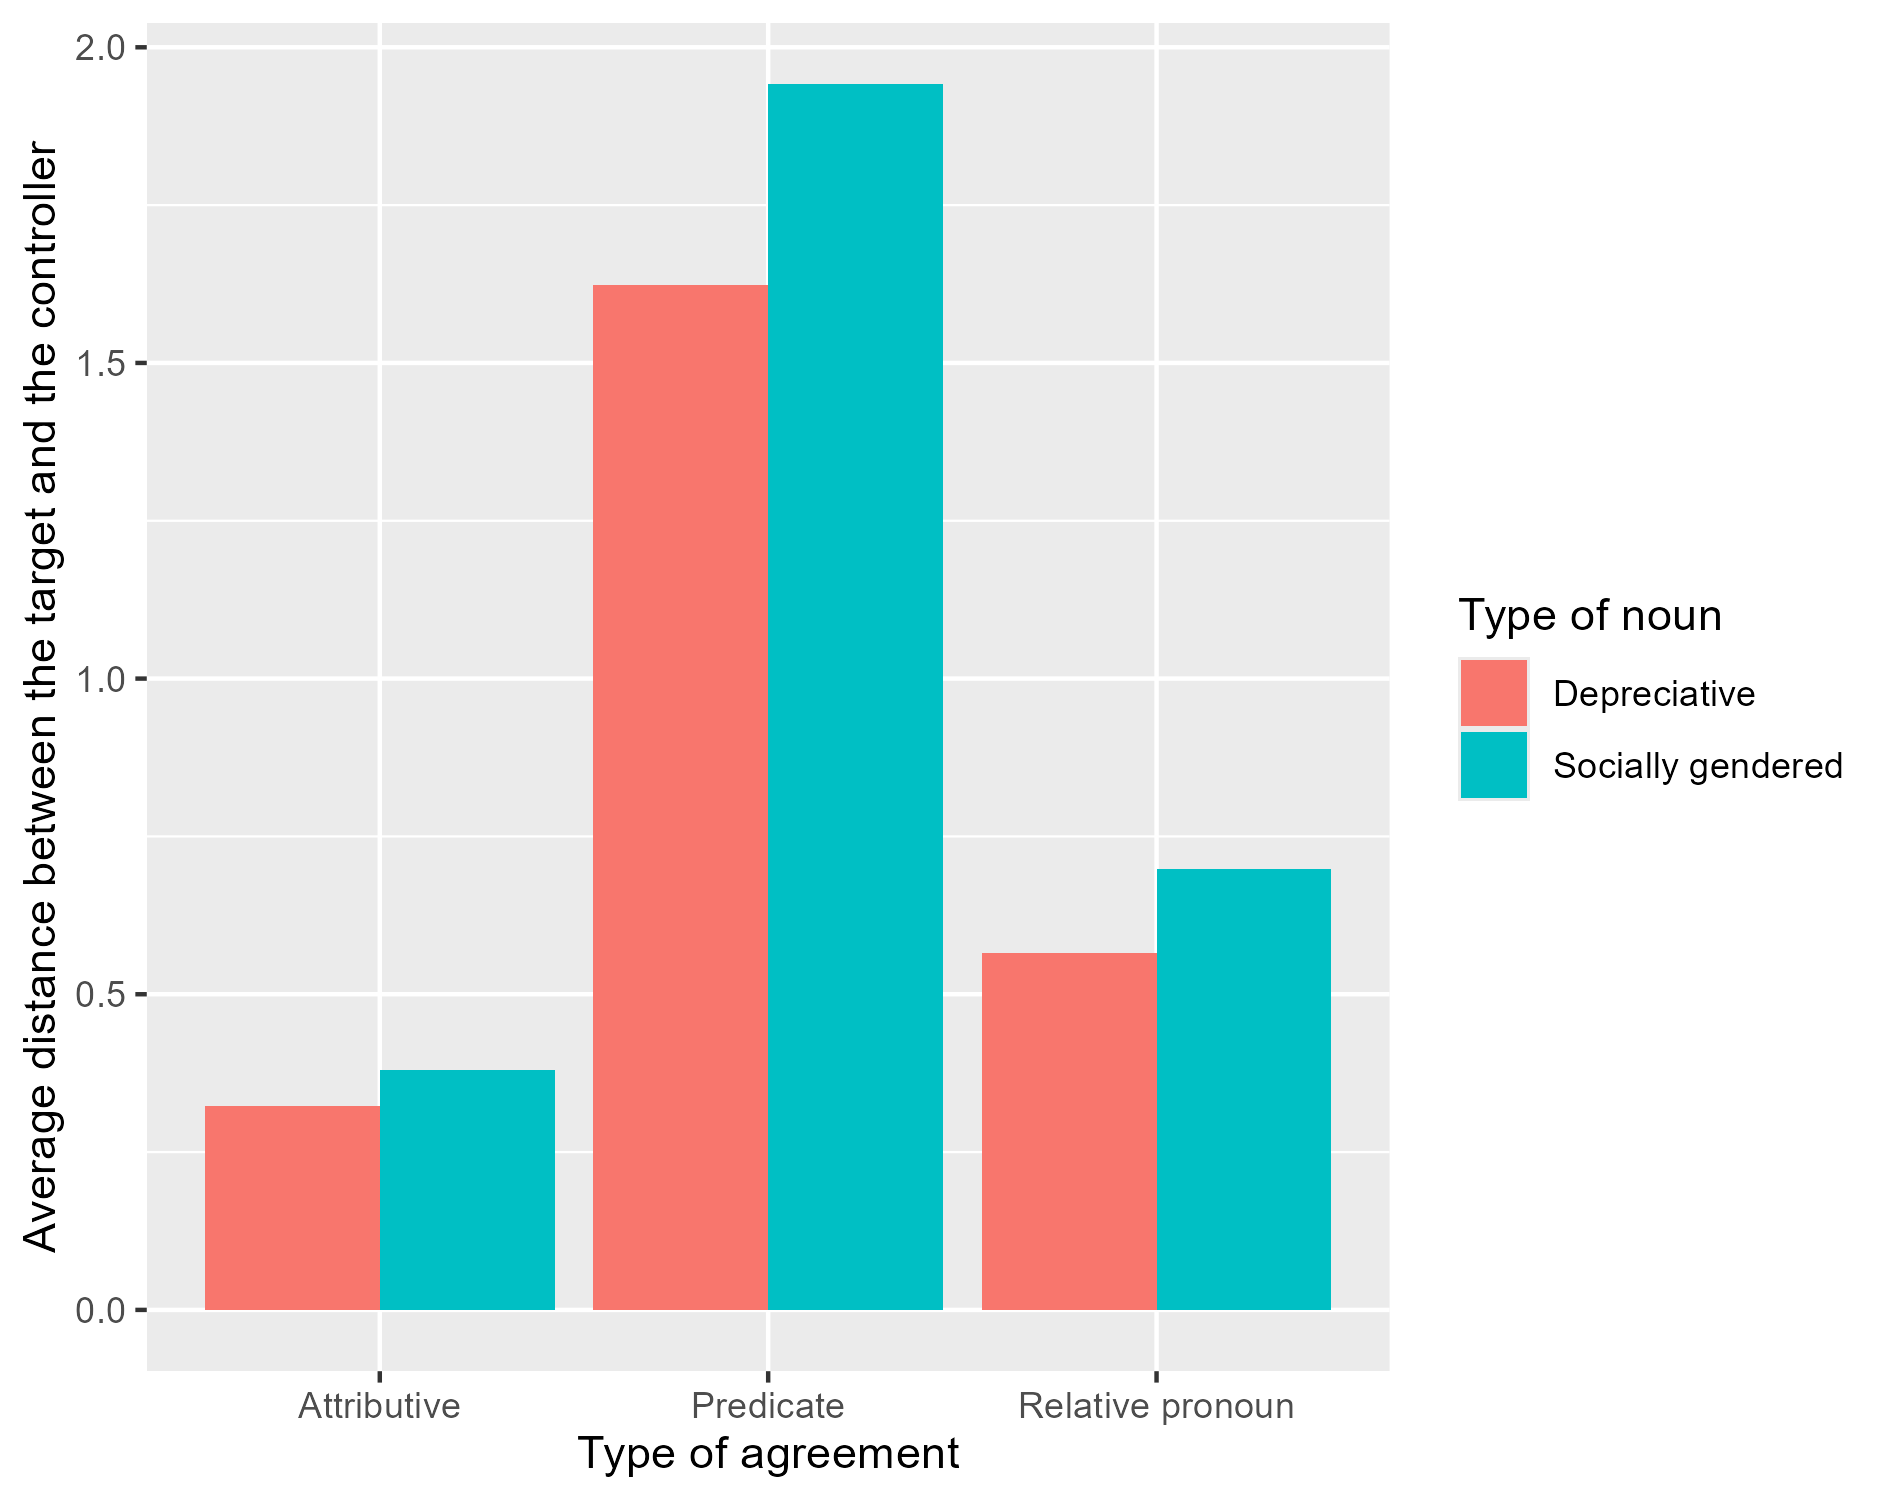
\includegraphics{images/dist.png}
  \caption{Average distance between the target and the controller of agreement for each type of agreement and for each type of noun.}
  \label{fig:distance}
\end{figure}

\begin{table}
  \centering
  \begin{tblr}
    {
      hlines,vlines,
      row{1} = gray9,
      cell{2}{1} = {r=2}{l},
      cell{4}{1} = {r=2}{l},
      cell{6}{1} = {r=2}{l},
    }
    Type of agreement & Type of noun & Average distance \\
    attributive & depreciative & 0.3223350 \\
    attributive & gendered & 0.3801262 \\
    predicative & depreciative & 1.6233333 \\
    predicative & gendered & 1.9416667 \\
    relpron & depreciative & 0.5652174 \\
    relpron & gendered & 0.6981132 \\
  \end{tblr}
  \caption{Average distance between the target and the controller in all types of nouns and agreements as shown in Figure \ref{fig:distance}.}
  \label{tab:distance}
\end{table}

As for the hypothesis regarding the hierarchy of agreement sources, 20.4\% of agreements with depreciatives had semantic agreement, while it was only 2.85\% for socially gendered nouns. This is further looked into in the following section.

It should be noted there were 15 profession nouns that did not have semantic agreement at all. Those nouns, along with their translations to English, can be found in Table \ref{tab:prof-zero}.

\begin{table}
  \centering
  \begin{tblr}
    {
      hlines, vlines,
      row{1} = {gray9},
      column{2} = {.4\hsize},
    }
    Lexeme in Polish & Translation to English & No. of occurrences \\
    demiurg & demiurge & 119 \\
    dramaturg & playwright & 397 \\
    elekt & person elected in a specified post, but has not yet entered office & 14 \\
    foniatra & phoniatrician & 2 \\
    ftyzjatra & pulmonologist & 1 \\
    geometra & geometer & 39 \\
    geriatra & geriatrician & 3 \\
    jaskiniowiec & caveman & 35 \\
    metalurg & metallurgist & 8 \\
    murarz & bricklayer & 241 \\
    muzykolog & musicologist & 80 \\
    nieuk & dunce & 37 \\
    nurek & diver & 109 \\
    pajac & clown & 10 \\
    szklarz & glazier & 50 \\
  \end{tblr}
  \caption{Table of profession nouns (and their translations and numbers of occurrences in the corpus), for which there was no semantic agreement found in the dataset.}
  \label{tab:prof-zero}
\end{table}
  
\section{Statistical models}

The models discussed in this section are not based on the profession nouns, since a vast amount of data in this category contained occurrences of the nouns that could not have hybrid agreement and could not have been filtered out automatically. The following analysis is based only on the agreements with depreciative forms and socially gendered nouns.

The analysis was conducted using the \texttt{glm} function from the \texttt{lme4} R package. Models computed using this function were all binomial generalized linear models, because the dependent variable was binary: whether semantic agreement was chosen or not. There were 4 variables tested as predictors for semantic agreement in separate generalized linear models. Those variables were: type of agreement (attrbutive, predicate, relative pronoun), distance between the target and the controller, target preceding the controller and type of controller noun (socially gendered or depreciative). No random factors were included. The formulae used for the models as well as the full output can be found in the Appendix. 

The model predicting based on the type of agreement showed that predicates favor semantic agreement more than attributives (estimate = -1.6722, p < 2e-16), but relative pronouns favor semantic agreement less than predicates (estimate = 1.0042, p = 0.0036), which does not show a monotonous shift from one value of gender to the other, as was expected. The model based on the distance gave expected results on the other hand, the larger the distance between the target and the controller, the more likely it is the semantic agreement will be chosen (estimate = 0.14115, p = 2.32e-06). According to the model predicting based on the ordering of the target and the controller, target being before the controller lowers the likelyhood of semantic agreement (estimate = -1.53658, p < 2e-16). Finally, the socially gendered nouns are less likely to have semantic agreement than the depreciatives (estimate = -2.1664, p < 2e-16).

Additionally, a multivariable model using the same 4 variables as predictors was computed. Estimates and p-values from this model are presented in Table \ref{tab:multivar-model}, the formula and full output of the model can be found in the Appendix. According to this model, when considering the interaction between all the predictors, only some of them are statistically significant. Predicate agreement favors semantic agreement, while socially gendered nouns do not. Target appearing before the controller also discourages from using semantic agreement.

\begin{table}[H]
  \centering
  \begin{tblr}
    {
      vlines,hlines,
      column{2,3} = {r},
      row{1} = {c, gray9},
    }
    Predictor & Estimate & P-value \\
    Predicate agreement & 0.45490 & \textbf{0.0345} \\
    Relative pronoun agreement & -0.21101 & 0.5959 \\
    Distance & 0.03983 & 0.2191 \\
    Ordering & -0.99116 & \textbf{1.59e-06} \\
    Type of noun: gendered & -1.73335 & \textbf{3.77e-13} \\
  \end{tblr}
  \caption{Estimates and p-values assigned to all predictors in the multivariable model. Predictors, that are statistically significant at the 0.05 level are bolded.}
  \label{tab:multivar-model}
\end{table}


	%% \chapter{Discussion}
\startcontents[chapters]

One of the surprising outcomes of the study is that there is no monotonous change from one value of gender to the other when going from attributive to relative pronoun agreement, which is contrary to one of the hypotheses. This may be a result of using low quality data for analysis -- the corpus, from which agreement was extracted, was first parsed automatically and the dependency trees produced this way have not been reviewed. It is possible that some of the words are annotated incorrectly or that there are non-existent dependencies found in the sentences.

It is also worth pointing out that there were very few instances of relative pronoun agreement -- 208 compared to 1478 and 1873 instances of predicate and attributive agreement respectively. In the univariable model predicting by type of agreement the difference between the relative pronoun and the predicate agreement is less significant than the difference between the predicate and attributive agreement, while the relative pronoun predictor in the multivariable model is not significant altogether. The unexpected decline in the proportion of semantic agreement between predicate and relative pronouns can be a result of limited relative pronoun data considered in the analysis. One of the possible directions for future research is to focus on hybrid agreement with relative and personal pronouns, since the current study offered little insight into those agreement targets.

There is also a potentially interesting observation to be made about the large mean distance between the target and controller of agreement, specifically in predicate agreement. The distance was found to be a significant predictor for semantic agreement (the larger the distance the more likely it is that semantic agreement will be chosen), but only by the univariable model. The multivariable model shows, that the effect of distance stops being statistically significant when other predictors are taken into account: one of the significant ones is predicative agreement. As a future perspective, it would be beneficial to test the predicative agreement with small distances between targets and controllers, to see if the preference for semantic agreement was here caused by large distance or by predicate targets.

\cite{corbett_agreement_1979} observed the ordering of the target and controller of agreement to have an influence over the choice between semantic and syntactic agreement -- this was found in the current study as well. According to both models, univariable and multivariable, if the target of agreement is placed before the controller it is unlikely that the agreement will be semantic. The effect is highly significant for both models.

Finally, another hypothesis tested here was that split hybrids are less likely to have semantic agreement than lexical hybrids. Depreciatives, which are an example of split hybrids, had semantic agreement in over 20\% of all occurrences, while the socially gendered nouns had semantic agreement in only 2.85\%, which is contrary to the expectations. It could be interesting to compare the depreciative forms with different split hybrids, to see it this preference for semantic agreement is exclusive to depreciatives or not. In an experimental study it would be possible to test the agreement with the Polish \textsl{ręka} (meaning 'hand') used by \cite{corbett_agreement_2023} to introduce split hybrids, since the examples in the corpus were not sufficient to do so in the present study. 

The corpus analysis yielded many occurrences of agreements with profession nouns, but unfortunately many of those were not useful for the present study. Without manually selecting the occurrences it was impossible to differentiate the examples where the referent was male from the ones where the referent was female, but all agreements were masculine. In the latter case it would have been an instance of hybrid agreement, where the speaker simply chose to use syntactic agreement for every target -- an interesting example that is technically possible, but could not have been selected automatically from the whole database of profession noun agreement. Nevertheless, the socially gendered nouns provided the opportunity to study Polish lexical hybrids, so the study was not harmed.

What should be noted, is that 15 of the profession nouns did not have any feminine agreements at all. Most of those words appeared in the corpus less than a 100 times each, the median of their number of occurrences in the corpus was 37. Since those nouns are rare, a better option would be to study them experimentally. There are no obvious feminitives for them \citep{szpyra-kozlowska_premiera_2019, szpyra-kozlowska_czy_2022}, therefore there is a high chance of finding hybrid agreement with them.


        %% \phantomsection
\chapter*{Conclusion}\label{chap:Conclusion}
\addcontentsline{toc}{chapter}{Conclusion}

The results of the study show, that with current evidence Corbett's Agreement Hierarchy and Hierarchy of Agreement Sources are not fully compatible with Polish data. The relative pronoun agreement was expected to have more semantic agreement than the predicates, but that was not the case in the analyzed data. This should be further investigated with experimental data, as very few examples of relative pronouns have been found in the corpus. According to the Hierarchy of Agreement Sources there should be more semantic agreement with lexical hybrids rather than with the split hybrids and the study found it to be the opposite. Additionally, profession nouns did not provide as much information as they potentaily could have, so further annotation is needed to use them for future analysis.


 %%%%%%%%%%%%%%%%%%%%%%%%%%%%%%%%%%%%%%%%%%%%%%%%%%%%%%%%%%%%%%%
 
        %\part{References}
        \phantomsection
        \chapter*{Bibliography}
        \addcontentsline{toc}{chapter}{Bibliography}
    
	\renewcommand{\bibsection}{}%to remove section in table of content
	\makeatletter
	\renewcommand\@biblabel[1]{}%to supress numbers
	\makeatother
	\vspace*{-40pt}
	
	%This is to supress URLs from the main bibliography!
	\bibliographystyle{apacite}
	\renewenvironment{APACrefURL}[1][]{}{}
	\AtBeginEnvironment{APACrefURL}{\renewcommand{\url}[1]{}}
	\renewcommand{\doiprefix}{doi:~\kern-1pt}
	\def\bibfont{\scriptsize}
		\bibliography{bibliography} % global bibliography
	
	%% \renewcommand*\listfigurename{List of figures}
	%% \listoffigures
	%% \addcontentsline{toc}{chapter}{List of figures}
	
	%% \renewcommand*\listtablename{List of tables}
	%% \listoftables
	%% \addcontentsline{toc}{chapter}{List of tables}
	
	\phantomsection
\chapter*{Appendices}\label{chap:Appendices}
\addcontentsline{toc}{chapter}{Appendices}

\begin{longtblr}[
caption = {Socially gendered and profession nouns in Polish and their translations or definitions in English},
label = {tab:noun-translations},
]{
hlines, vlines,
rowhead = 1,
row{1} = {gray9},
column{1} = {.2\hsize},
column{2} = {.45\hsize},
column{3} = {.15\hsize},
}
Noun in Polish & Translation or definition in English & Category\\
adiunkt & someone who holds a PhD title and is employed at a scientific institution & profession\\
architekt & architect & profession\\
babochłop & a woman that resembles a man with her physicality, looks and behavior & gendered\\
babol & a woman that looks or behaves in a way that causes aversion in the speaker & gendered\\
babon & a woman, about whom the speaker feels negatively & gendered\\
babsko & a woman, about whom the speaker feels negatively & gendered\\
babsztyl & a woman, about whom the speaker feels negatively & gendered\\
babus & a woman, about whom the speaker feels negatively & gendered\\
burmistrz & mayor & profession\\
chirurg & surgeon & profession\\
chłopaczysko & a tall or big young man & gendered\\
chłopobaba & a man that resembles a woman with his physicality, looks and behavior (can also mean a woman that resembles a man) & gendered\\
ciota & a homosexual man (can also refer to a woman about whom the speaker feels negatively) & gendered\\
demiurg & demiurge & profession\\
dramaturg & playwright & profession\\
drań & scoundrel & profession\\
dupek & asshole & profession\\
dureń & fool & profession\\
dziekan & dean & profession\\
dziewczątko & a girl, whom the speaker likes or to whom they feel compassion & gendered\\
dziewczę & a young girl & gendered\\
dziewuszysko & a girl who causes aversion or contempt in the speaker & gendered\\
ekspert & expert & profession\\
elekt & person elected in a specified post, but has not yet entered office & profession\\
foniatra & phoniatrician & profession\\
ftyzjatra & pulmonologist & profession\\
geometra & geometer & profession\\
geriatra & geriatrician & profession\\
ginekolog & gynecologist & profession\\
głupek & fool & profession\\
herszt & ringleader & profession\\
inżynier & engineer & profession\\
jaskiniowiec & caveman & profession\\
jeniec & captive & profession\\
jeździec & rider & profession\\
kierowca & driver & profession\\
kobiecisko & expressively about a woman, augumentative, or to refer to a big woman & gendered\\
kobieciątko & expressively about a woman, diminutive & gendered\\
kobieton & a woman that resembles a man with her physicality, looks and behavior & gendered\\
ksiądz & priest & profession\\
lump & tramp & profession\\
magister & master (holder of a university degree) & profession\\
majster & foreman & profession\\
metalurg & metallurgist & profession\\
minister & minister & profession\\
murarz & bricklayer & profession\\
muzykolog & musicologist & profession\\
mędrzec & wise man & profession\\
naukowiec & scientist & profession\\
nieuk & dunce & profession\\
nurek & diver & profession\\
pacholę & a boy & gendered\\
pajac & clown & profession\\
pannisko & expressively about a young woman, augumentative & gendered\\
pastor & pastor & profession\\
pasztet & an ugly and unattractive woman & gendered\\
pediatra & pediatrician & profession\\
petent & applicant & profession\\
polityk & politician & profession\\
porucznik & lieutenant & profession\\
powstaniec & insurgent & profession\\
prefekt & prefect & profession\\
premier & prime minister & profession\\
prezydent & president & profession\\
proboszcz & parish priest & profession\\
psychiatra & psychiatrist & profession\\
pułkownik & colonel & profession\\
rektor & person in charge of a university & profession\\
sierżant & sargeant & profession\\
starosta & highest administrative officer of a second-level unit of local government & profession\\
subiekt & salesman & profession\\
szklarz & glazier & profession\\
szpieg & spy & profession\\
szubrawiec & rascal & profession\\
upiór & phantom & profession\\
wamp & a confident, misterious, provocative and attractive woman who seduces men & gendered\\
widz & audience member & profession\\
wójt & highest administrative officer of a basic-level unit of local government & profession\\
zbieg & fugitive & profession\\
\end{longtblr}


\begin{figure}[H]
\footnotesize
\typewriting{
\verbatiminput{Chapters/typeofagreement.txt}
}
\caption{Output of the model based on type of agreement.}
\end{figure}

\begin{figure}[H]
\footnotesize
\typewriting{
\verbatiminput{Chapters/distance.txt}
}
\caption{Output of the model based on distance.}
\end{figure}

\begin{figure}[H]
\footnotesize
\typewriting{
\verbatiminput{Chapters/ordering.txt}
}
\caption{Output of the model based on the order of the target and the controller.}
\end{figure}

\begin{figure}[H]
\footnotesize
\typewriting{
\verbatiminput{Chapters/controller.txt}
}
\caption{Output of the model based on type of controller.}
\end{figure}

\begin{figure}[H]
\footnotesize
\typewriting{
\verbatiminput{Chapters/multivariable.txt}
}
\caption{Output of the multivariable model.}
\end{figure}


	%% \phantomsection
\chapter*{Autorisation for publishing and reusing documents}\label{chap:Autorisations}
\addcontentsline{toc}{chapter}{Autorisation for publishing and reusing documents}


\end{document}
